% Compile twice with pdfLaTeX from this directory.
% Keep beamerthemeHeidelberg.sty here and 2408.03314v1.pdf one directory above.
\documentclass[aspectratio=1610,xcolor=dvipsnames,t]{beamer}
\usepackage{lmodern}
\usepackage{sansmath}
\usepackage{mathastext}
\usepackage{graphicx}
\usepackage{beamerthemesplit}
\usetheme[compress]{Heidelberg}
\definecolor{unirot}{rgb}{0.5976525,0,0}
\usecolortheme[named=unirot]{structure}
\usepackage{amsmath,amssymb}

\newcommand{\keyterm}[1]{\textcolor{unirot}{\textbf{#1}}}
\setbeamertemplate{headline}{}
\newcommand{\papersource}[1]{\par\smallskip{\scriptsize\color{gray} Snell et al. (2024), #1\par}}
% Arguments: source page, viewport in PDF points, displayed width.
\newcommand{\paperfig}[3]{%
  \includegraphics[page=#1,viewport=#2,clip,width=#3,height=.47\textheight,keepaspectratio]{../2408.03314v1.pdf}%
}

\title[Test-Time Compute in LLMs]{Scaling LLM Test-Time Compute Optimally can be More Effective than Scaling Model Parameters}
\subtitle{How should a model spend its inference budget?}
\author[Presenter]{Zhenbang Lyu}
\institute[Uni HD]{Heidelberg University\\Institute of Computer Science}
\date{Snell, Lee, Xu, and Kumar (2024)}


\begin{document}
\begin{frame}[plain]
  \titlepage
\end{frame}

\begin{frame}{You Have 16 More Generations}
  A model tries to solve a competition math problem and gives the wrong answer. Where should the next 16 generations go?
  \medskip
  \begin{columns}[T,onlytextwidth]
    \begin{column}{.48\textwidth}
      \begin{block}{Right approach, wrong arithmetic}
        The model sets up the right equation but makes a sign error. A revision could fix it.
      \end{block}
    \end{column}
    \begin{column}{.48\textwidth}
      \begin{block}{Wrong approach}
        The model assumes a relationship the problem never gives. A fresh attempt could find a better setup.
      \end{block}
    \end{column}
  \end{columns}
  \medskip
  A verifier can also score partial solutions and decide which ones to develop further.
\end{frame}

\begin{frame}{Three Ways to Spend the Budget}
  \begin{enumerate}
    \item \textbf{Sample independently.} Generate full solutions in parallel. Use weighted best-of-$N$ to select a final answer.
    \item \textbf{Revise sequentially.} Generate a new attempt conditioned on earlier ones. Split the budget across multiple chains if exploration also matters.
    \item \textbf{Search with a verifier.} Use a process reward model (PRM) to score partial solutions. Beam search expands the highest-scoring prefixes. Lookahead first generates extra steps before scoring.
  \end{enumerate}
  \begin{block}{Two places to intervene}
    Revisions change what the model proposes. Verifier search changes which proposals get more compute.
  \end{block}
  \papersource{Sections 2, 5 and 6.}
\end{frame}

\begin{frame}{Difficulty Is Relative to the Model}
  The study uses PaLM 2-S* on 500 MATH test problems. It fine-tunes models for verification and revision.
  \begin{itemize}
    \item \textbf{Oracle difficulty} \quad Estimate the model's chance of solving each problem from 2,048 attempts. Group the questions into five difficulty bins.
    \item \textbf{Predicted difficulty} \quad Use the verifier's mean score in place of known correctness.
    \item \textbf{Adaptive policy} \quad At each budget, select the best setting for each difficulty bin on one fold and evaluate it on the other. Swap folds and average.
  \end{itemize}
  \begin{alertblock}{Cost left out of the comparison}
    The reported generation budgets exclude the cost of estimating difficulty.
  \end{alertblock}
  \papersource{Sections 3--4.}
\end{frame}

\begin{frame}{Beam Search Helps When the Budget Is Small}
  \begin{center}
    \paperfig{9}{61 539 551 708}{.98\textwidth}
  \end{center}
  \small
  \begin{itemize}
    \item Beam search leads at low budgets. Lookahead generally trails at the same estimated cost.
    \item At higher budgets, beam search can hurt in easy bins 1--2, where it can amplify verifier errors. It helps in bins 3--4.
    \item The hardest bin shows little improvement across methods.
  \end{itemize}
  \papersource{Section 5.3 and Figure 3.}
\end{frame}

\begin{frame}{How the Revision Model Uses Earlier Attempts}
  \begin{center}
    \paperfig{11}{62 525 549 709}{.98\textwidth}
  \end{center}
  \small
  \begin{itemize}
    \item During training, the model learns to produce a correct solution given up to four related incorrect attempts.
    \item At test time, a revision can undo a correct solution. The paper selects among attempts with a verifier or majority vote.
  \end{itemize}
  \papersource{Section 6.1 and Figure 5.}
\end{frame}

\begin{frame}{Easy Problems Benefit from Longer Revision Chains}
  \begin{center}
    \paperfig{13}{61 539 551 708}{.98\textwidth}
  \end{center}
  \begin{itemize}
    \item \textbf{Left} \quad As the budget grows, a mix of parallel and sequential compute can beat either extreme.
    \item \textbf{Right} \quad At 128 generations, easy problems favor a single chain. Harder problems often benefit from multiple starting points.
  \end{itemize}
  \papersource{Section 6.2 and Figure 7.}
\end{frame}

\begin{frame}{What Does Difficulty-Based Allocation Buy?}
  \begin{columns}[T,onlytextwidth]
    \begin{column}{.48\textwidth}
      \centering
      \paperfig{10}{306 466 551 635}{\linewidth}
      \par\smallskip
      {\small\keyterm{Search}\quad 16 generations nearly match 64 with PRM best-of-$N$.}
    \end{column}
    \begin{column}{.48\textwidth}
      \centering
      \paperfig{13}{306 186 551 357}{\linewidth}
      \par\smallskip
      {\small\keyterm{Revisions}\quad 64 generations beat 256 with parallel best-of-$N$.}
    \end{column}
  \end{columns}
  \medskip
  \papersource{Figures 4 and 8. These are generation-budget comparisons.}
\end{frame}

\begin{frame}{Equal Total FLOPs, Two Ways to Spend Them}
  Compare a larger model decoding greedily with a smaller model using adaptive inference. The paper holds pretraining tokens fixed and increases parameter count by about $14\times$.
  \[
    \underbrace{X+aY}_{\text{smaller model, more inference}}
    =
    \underbrace{M(X+Y)}_{\text{larger model, greedy decoding}}
  \]
  \begin{itemize}
    \item $X$ and $Y$ are the smaller model's baseline pretraining and inference FLOPs. $M$ scales its parameter count and $a$ scales its inference compute.
    \item $R$ is total inference tokens divided by pretraining tokens. When $R$ is low, the smaller model can spend more compute per inference token at the same total cost.
  \end{itemize}
  \papersource{Section 7.}
\end{frame}

\begin{frame}{Reading the FLOPs Comparison}
  \begin{center}
    \paperfig{15}{64 526 549 715}{.98\textwidth}
  \end{center}
  \small
  \begin{itemize}
    \item \textbf{Line} \quad Accuracy as the smaller model spends more on adaptive inference in one difficulty bin.
    \item \textbf{Star} \quad Greedy accuracy of the larger model, placed at the matching FLOPs budget for that workload.
    \item A line above its matching star favors the smaller model.
  \end{itemize}
  \papersource{Section 7 and Figure 9.}
\end{frame}

\begin{frame}{When Is a Larger Model Worth the Compute?}
  \begin{columns}[T,onlytextwidth]
    \begin{column}{.48\textwidth}
      \begin{block}{Extra inference often wins}
        Easier or intermediate problems, where the smaller model already has some chance of success. A low inference workload makes more extra compute available per request.
      \end{block}
    \end{column}
    \begin{column}{.48\textwidth}
      \begin{block}{A larger model often wins}
        The hardest problems, where revisions and search make little progress, or a high inference workload, where extra compute per request adds up.
      \end{block}
    \end{column}
  \end{columns}
  \medskip
  The study tests workload ratios $R=0.16$, $0.79$, and $22$.
  \papersource{Section 7 and Figure 9.}
\end{frame}

\begin{frame}{What the Experiment Leaves Open}
  \begin{itemize}
    \item \textbf{Difficulty at deployment} \quad How much of the inference budget should we spend estimating difficulty before trying to solve the problem?
    \item \textbf{Transfer} \quad The study uses PaLM 2-S* on MATH. Other models and tasks can change which problems are within reach.
    \item \textbf{Combining methods} \quad The paper tests verifier-based selection among revisions. Combining PRM tree search with revision chains remains open.
  \end{itemize}
  \papersource{Sections 3.2 and 8.}
\end{frame}

\begin{frame}{Back to the 16 Generations}
  \begin{itemize}
    \item \textbf{A promising approach} \quad Spend more of the budget revising it.
    \item \textbf{Several plausible approaches} \quad Try more starting points or use a verifier to guide search.
    \item \textbf{Almost no successful attempts} \quad In these experiments, more generations rarely close the gap.
  \end{itemize}
  \medskip
  \begin{block}{The practical question}
    Can we recognize which situation we are in cheaply enough to choose a strategy?
  \end{block}
\end{frame}

\begin{frame}{Questions}
  \vfill
  \begin{center}
    {\Huge\color{unirot}\textbf{Thank you.}}\\[0.4cm]
    {\Large Questions and Discussion}
  \end{center}
  \vfill
\end{frame}

\end{document}

